\documentclass[SE,lsstdraft,authoryear,toc]{lsstdoc}
\input{meta}

% Package imports go here.
\usepackage{subcaption}                 % supports \begin{subfigure}...\end{subfigure}
\usepackage{xspace}

% Local commands go here.
\newcommand{\ComCam}{ComCam\xspace}
\setlength{\headheight}{62pt}           % heed warnings that these values need adjusting
\addtolength{\topmargin}{-7pt}

%If you want glossaries
%\input{aglossary.tex}
%\makeglossaries

\title{An Interim Report on the ComCam On-Sky Campaign}

% This can write metadata into the PDF.
% Update keywords and author information as necessary.
\hypersetup{
    pdftitle={An Interim Report on the ComCam On-Sky Campaign},
    pdfauthor={Robert Lupton},
    pdfkeywords={}
}

% Optional subtitle
% \setDocSubtitle{A subtitle}

\author{%
Many authors
}

\setDocRef{SITCOMTN-149}
\setDocUpstreamLocation{\url{https://github.com/lsst-sitcom/sitcomtn-149}}

\date{\vcsDate}

% Optional: name of the document's curator
% \setDocCurator{The Curator of this Document}

\setDocAbstract{%
A summary of what we have learned from the initial period of ComCam observing
}

% Change history defined here.
% Order: oldest first.
% Fields: VERSION, DATE, DESCRIPTION, OWNER NAME.
% See LPM-51 for version number policy.
\setDocChangeRecord{%
  \addtohist{1}{YYYY-MM-DD}{Unreleased.}{Robert Lupton}
}


\begin{document}

% Create the title page.
\maketitle
% Frequently for a technote we do not want a title page  uncomment this to remove the title page and changelog.
% use \mkshorttitle to remove the extra pages

% ADD CONTENT HERE
% You can also use the \input command to include several content files.

\section{Introduction}
\label{sec:introduction}

The Vera C. Rubin Observatory on-sky commissioning campaign using the Commissioning Camera (ComCam) began on 24 October 2024 and is forecasted to continue through mid-December 2024.
This interim report provides a concise summary of our understanding of the integrated system performance based tests and analyses conducted during the first weeks of the ComCam on-sky campaign.
The emphasis is distilling and communicating what we have learned about the system.
The report is organized into sections to describe major activities during the campaign, as well as multiple aspects of the demonstrated system and science performance.

\subsection{Charge}

We identify the following high-level goals for the interim report:

\begin{itemize}

    \item \textbf{Rehearse workflows for collaboratively developing documentation} to describe our current understanding of the integrated system performance, e.g., to support the development of planned Construction Papers and release documentation to support the Early Science Program \citedsp{RTN-011}.
    This report represents an opportunity to collectively exercise the practical aspects of developing documentation in compliance with the policies and guidelines for information sharing during commissioning \citedsp{sitcomtn-076}.

    \item \textbf{Synthesize the new knowledge} gained from the ComCam on-sky commissioning campaign to inform the optimization of activities between the conclusion of the ComCam campaign and the start of the on-sky campaign with the LSST Camera (LSSTCam).

    \item \textbf{Inform the Rubin Science Community} on the progress of the on-sky commissioning campaign using ComCam.

\end{itemize}

Other planned systems engineering activities will specifically address system-level verification (\citedsp{lse-29} and \citedsp{lse-30}) using tests and analysis from the ComCam campaign.
While the analyses in this report will likely overlap with the generation of verification artifacts for systems engineering, and system-level requirement specifications will serve as key performance benchmarks for interpreting the progress to date, formal acceptance testing is not an explicit goal of this report.

\textbf{The groups within the Rubin Observatory project working on each of the activities and performance analyses are charged with contributing to the relevant sections of the report.}
The anticipated level of detail for the sections ranges from a paragraph up to a page or two of text, depending on the current state of understanding, with quantitative performance expressed as summary statistics, tables, and/or figures.
The sections refer to additional supporting documentation, e.g., analysis notebooks, other technotes with further detail, as needed.

The anticipated timeline for developing this interim report are as follows:

\begin{itemize}

    \item 18 Nov 2024: Define charge

    \item 4 Dec 2024: First drafts of report sections made available for internal review

    \item 11 Dec 2024: Revised drafts of report sections made available for internal review; editing for consistency and coherency throughout the report

    \item 18 Dec 2024: Initial version of report is released

\end{itemize}

\begin{warning}[On-sky Pixel Image Embargo]
    All pixel images and representations of pixel images of any size field of view, including individual visit images, coadd images, and difference images based on ComCam commissioning on-sky observations must be kept internal to the Rubin Observatory Project team, and in particular, cannot be included in this report.
    Embargoed pixel images can only be referenced as authenticated links.
    See \citedsp{sitcomtn-076} for details.
\end{warning}

\section{System Performance Analysis}
\label{sec:system_performance_analysis}

\newcommand{\TMAMotionSettings}{\href{https://rubinobs.atlassian.net/wiki/spaces/LSSTCOM/pages/53741249/TMA+Motion+Settings}{TMA Motion Settings}}

Topics to convert into text

\begin{itemize}
    - M1M3 and M2 glass installed on the Simonyi Survey Telescope.
    - Since then, we have been operating the telescope with limited velocity,
    acceleration, and jerk limits following the performances defined in \TMAMotionSettings.
    - For each configuration, defined in terms of a percentage of the maximum
    velocity, acceleration, and jerk, we ran multiple gateway tests.
    - The gateway tests are described in the subsection \ref{subsec:gateway_tests} below.
\end{itemize}

\subsection{Gateway Tests}

The three gateway tests defined below are required for each increase in the
velocity, acceleration, and jerk limits. They are associated with glass and
telescope safety. So far, we have been able to run the telescope up to 10\%
its maximum velocity, acceleration, and jerk limits. For simplicity, we will
show only the last results.


\subsubsection{Long and short slews at different elevations}
\label{subsubsec:long_and_short_slews}

These tests ensure that the force balance systems on M1M3 and on M2 can protect
the mirrors on different telescope positions and while slewing. As we increase
velocity, acceleration, and jerk limits, both mirrors suffer higher inertial
forces and the force actuators must counteract them.

For M1M3, the criteria is to keep the measured forces on the hardpoint actuators
below the operational limit (15\% the breakaway limit). For M2, the criteria is
??????? (check with Holger, Gabriele, and Pablo). % TODO - check with

Test cases associated:
\begin{itemize}
    - \href{https://rubinobs.atlassian.net/projects/BLOCK?selectedItem=com.atlassian.plugins.atlassian-connect-plugin:com.kanoah.test-manager__main-project-page#!/v2/testCase/BLOCK-T227}{BLOCK-T227 Dynamic Tests at El = 34º - short and long slews}
    - \href{https://rubinobs.atlassian.net/projects/BLOCK?selectedItem=com.atlassian.plugins.atlassian-connect-plugin:com.kanoah.test-manager__main-project-page#!/v2/testCase/BLOCK-T293}{BLOCK-T293 Dynamic Tests at El = 70º - short and long slews}
    - \href{https://rubinobs.atlassian.net/projects/BLOCK?selectedItem=com.atlassian.plugins.atlassian-connect-plugin:com.kanoah.test-manager__main-project-page#!/v2/testCase/BLOCK-T294}{BLOCK-T294 Dynamic Tests at El = 70º - short and long slews}
    - \href{https://rubinobs.atlassian.net/projects/LVV?selectedItem=com.atlassian.plugins.atlassian-connect-plugin:com.kanoah.test-manager__main-project-page#!/v2/testCase/LVV-T2813}{LVV-T2813 M1M3 Dynamic Test, increasing speed, increasing acceleration}
    - \href{https://rubinobs.atlassian.net/projects/LVV?selectedItem=com.atlassian.plugins.atlassian-connect-plugin:com.kanoah.test-manager__main-project-page#!/v2/testCase/LVV-T2944}{LVV-T2944 M2 Dynamic Test, increasing speed, acceleration, jerk}
\end{itemize}

Detailed analysis (both TNs are still under development):
\begin{itemize}
    - \href{https://sitcomtn-092.lsst.io/}{SITCOM-TN092 M1M3 Force Balance System - Inertia Compensation}
    - \href{https://sitcomtn-147.lsst.io/}{SITCOM-TN147 M2 Response to short and long slews}
\end{itemize}

\begin{figure}
    \centering
    \includegraphics[width=0.8\textwidth]{spa/M1M3_short_long_slews_10_histogram.png}
    \caption{Number of slews with minimum/maximum measured forces on the M1M3 hardpoint actuators.}
    \label{fig:m1m3_short_long_slews}
    \end{figure}

\begin{figure}
    \centering
    \includegraphics[width=0.8\textwidth]{spa/M2_short_long_slews_axial_measured_force_10.png}
    \caption{Measured axial force on the M2 force actuators during short and long slews.}
    \label{fig:m2_short_long_slews_axial}
    \end{figure}

\begin{figure}
    \centering
    \includegraphics[width=0.8\textwidth]{spa/M2_short_long_slews_Tangent_measured_forces_TMA_10.png}
    \caption{Measured tangent force on the M2 force actuators during short and long slews.}
    \label{fig:m2_short_long_slews_tangent}
    \end{figure}

\begin{figure}
    \centering
    \includegraphics[width=0.8\textwidth]{spa/M2_short_long_slews_tangent_force_errors_10.png}
    \caption{Measured tangent force errors on the M2 force actuators during short and long slews.}
    \label{fig:m2_short_long_slews_tangent_errors}
    \end{figure}


\subsubsection{M2 close-loop breakout tests}
\label{subsubsec:m2_close_loop_breakout_tests}

\begin{itemize}
    - \href{https://rubinobs.atlassian.net/projects/LVV?selectedItem=com.atlassian.plugins.atlassian-connect-plugin:com.kanoah.test-manager__main-project-page#!/v2/testCase/LVV-T3034}{LVV-T3034 M2 closed-loop break-out during TMA slew}
    - \href{https://rubinobs.atlassian.net/projects/BLOCK?selectedItem=com.atlassian.plugins.atlassian-connect-plugin:com.kanoah.test-manager__main-project-page#!/v2/testCase/BLOCK-T241}{BLOCK-T241 M2 closed-loop break-out brake test during TMA slew}
\end{itemize}

\begin{figure}
    \centering
    \includegraphics[width=0.8\textwidth]{spa/M2_cl_breakout_10_axial_force.png}
    \caption{M2 axial forces during the closed-loop breakout test.}
    \label{fig:m2_closed_loop_breakout_axial_force}
    \end{figure}

\begin{figure}
    \centering
    \includegraphics[width=0.8\textwidth]{spa/M2_cl_breakout_10_tangent_forces.png}
    \caption{M2 tangent forces during the closed-loop breakout test.}
    \label{fig:m2_closed_loop_breakout_tangent_force}
    \end{figure}

\begin{figure}
    \centering
    \includegraphics[width=0.8\textwidth]{spa/M2_cl_breakout_10_tangent_force_errors.png}
    \caption{M2 tangent force errors during the closed-loop breakout test.}
    \label{fig:m2_closed_loop_breakout_tangent_force_errors}
    \end{figure}


\subsubsection{TMA azimuth and elevation brake tests}
\label{subsubsec:tma_azimuth_and_elevation_brake_tests}

Test cases associated:
\begin{itemize}
    - \href{https://rubinobs.atlassian.net/projects/BLOCK?selectedItem=com.atlassian.plugins.atlassian-connect-plugin:com.kanoah.test-manager__main-project-page#!/v2/testCase/BLOCK-T231}{BLOCK-T231 TMA Azimuth Brake Test}
    - \href{https://rubinobs.atlassian.net/projects/BLOCK?selectedItem=com.atlassian.plugins.atlassian-connect-plugin:com.kanoah.test-manager__main-project-page#!/v2/testCase/BLOCK-T240}{BLOCK-T240 TMA Elevation Brake Distance}
\end{itemize}

\begin{figure}
    \centering
    \includegraphics[width=0.8\textwidth]{spa/TMA_Az_brake_test_10.png}
    \caption{TMA azimuth brake test.}
    \label{fig:tma_azimuth_brake}
    \end{figure}

\begin{figure}
    \centering
    \includegraphics[width=0.8\textwidth]{spa/TMA_El_brake_test_10.png}
    \caption{TMA elevation brake test.}
    \label{fig:tma_elevation_brake}
    \end{figure}


\section{Active Optics System Commissioning}
\label{sec:aos_commissioning}

The commissioning of the Active Optics System (AOS) has marked a significant milestone for the Rubin Observatory, 
demonstrating the system's readiness to support high-quality imaging. The first images captured with ComCam 
achieved an impressive 1.7 arcsecond full-width half-maximum (FWHM) image quality, exceptional work of the engineering 
and optical teams during assembly and to the optimization of the Look-Up Table (LUT) using laser tracker data at
the beginning of 2024. Through rigorous testing, frustration and lots of learning, 
we have achieved a system capable of delivering sub-arcsecond image quality with good seeing, 
laying the foundation for the transition to LSSTCam commissioning and the start of survey operations.

\subsection{Initial Alignment}
The initial alignment of the AOS utilized an updated laser tracker nominal frame, ensuring the system was 
consistently brought into focus. These refinements simplified the alignment process, demonstrating the 
value of accurate laser tracker data and paving the way for seamless operations.

\subsection{Coordinate Systems}
Throughout commissioning, significant effort was devoted to understanding and refining coordinate systems. 
We identified a rotation discrepancy in ComCam's installation compared to the expected design, requiring 
adjustments in our alignment procedures. This experience was useful to prepare for similar challenges 
with LSSTCam, equipping the AOS team with strategies to handle future discrepancies.

\subsection{Wavefront estimation}
The wavefront estimator proved robust across diverse observing conditions. 
On dense fields such as 47 Tuc, the estimator provided accurate results for 
all sensors except the central one. Validation against Batoid simulations confirmed 
the good accuracy of Rubin's ray-tracing software.

Advancements included the implementation of sparse Zernikes, which allowed selective 
inclusion of terms while minimizing cross-correlations of modes with identical azimuthal 
dependencies. The forward-model approach (Danish) demonstrated resilience to poor seeing 
and significant defocus, although it remains slower than the TIE method. Improving the 
computational efficiency of both techniques remains a priority for the team.

\subsection{Closed Loop}
Following resolution of initial issues with the AOS pipelines, 
closed-loop operations were achieved across varying elevations. 
Most optical modes were utilized, excluding the three highest-order modes on M2. 
Consistency in results across nights confirmed the need for further refinement of the LUT.

In favorable seeing conditions, the system achieved sub-arcsecond image 
quality, with FWHM as low as 0.65 arcseconds. Zernike-based AOS FWHM 
contributions confirmed the system's convergence to exceptional image 
quality. Autonomous closed-loop operations were run by observers, 
demonstrating the maturity of the system. Preparations are underway 
for a fully autonomous survey-mode triplet-taking block before the 
conclusion of ComCam's on-sky operations.

\subsection{LUT}
The LUT underwent initial validation across elevations, azimuths, and rotator angles, 
leading to incremental improvements. While these updates enhanced performance, 
further refinements are needed to address second-order dependencies. Insights 
from ComCam data will inform these efforts, ensuring readiness for LSSTCam, which 
may present distinct challenges due to its larger focal plane and optical system.

\subsection{Lessons Learned and Next Steps}
\textbf{Lessons Learned}
- Coordinate Systems: Precision and methodical testing of coordinate systems are essential. 
Starting with foundational tests and incrementally increasing complexity ensures reliability.
- Observer Training: Comprehensive documentation, including a subsystem overview and closed-loop procedures, 
significantly enhances observer support capabilities.
- Engagement and Morale: Fun and engaging night summaries boost team morale, fostering a collaborative 
and motivated work environment.
- Transferability: Some ComCam learnings, particularly LUT and coordinate system adjustments, 
will not fully transfer to LSSTCam, requiring repeated validation.

\textbf{Next Steps}
- Conduct step-by-step closed-loop validations for LSSTCam, validating signs and rotations for intentional perturbations.
- Collaborate with the Camera Team to anticipate and mitigate known camera tilts.
- Implement and validate tests tailored to LSSTCam's larger focal plane dimensions.
- Prepare RubinTV and donutViz for full-array LSSTCam mode and automate its execution for all triplet-taking sequences.
- Adapt MTAOS to run as a continuous background task, supporting survey-mode operations.
- Optimize the AOS pipeline for speed, including binning and ISR performance improvements.




\section{Image Quality}
\label{sec:image_quality}

The AOS team has delivered very impressive image quality, showing images with 0.68 arcsec FWHM. If we assume that sources of image degradation add in quadrature and we trust our estimates of atmospheric seeing, this is consistent with reaching the image quality error budget allocation of our full system of 0.400 arcsec.

We are in the process of quantifying the different sources of image degradation. The main ones we're focused on measuring are degradation due to the camera/instrument, static optics, dynamic optics, mount motion, and observatory seeing.

\subsection{Atmospheric Seeing}

We do not currently have a working Rubin DIMM, although there repairs are in progress. In the meantime, we have a livestream of data from the SOAR RINGS instrument, which is a  next-generation DIMM developed by Andrei Tokovinin and Edison Bustos. We are working on getting direct access to current and historical data for RINGS as well as the Gemini DIMM. This access will make it much easier to quantify the different sources of image degradation.

\subsection{Static Optics}

See Section~\ref{sec:aos_commissioning} for more details on the performance of the static optics system.

\subsection{Instrument}

We are taking the measured LSSTCam instrument image degradation to be the same as for ComCam, so we will use budget table developed at SLAC.

\subsection{Dynamic Optics}

Dynamic optics contributions are caused by oscillations or motion of the mirrors, causing focus to shift during an exposure. We have accelerometers in the mirror cell and on the top end but have not yet analyzed the data.

\subsection{Observatory Seeing}

The two main contributors to observatory seeing are dome seeing and mirror seeing. We do not have a direct dome seeing monitor but we do have a 3D sonic anemometer located in the dome that is taking data. Larom Segev has looked at the correlation between the standard deviation of the sonic temperature, which should be a proxy for dome seeing due to thermal turbulence, and measured PSF FWHM in the science images (see Fig.~\ref{fig:anemometer}). There may be some correlation, but we need more and better data, and to remove atmospheric seeing contributions.

\begin{figure}
    \includegraphics[width=\linewidth]{image_quality_figures/anemometer_PSF.png}
    \caption{PSF FWHM versus the standard deviation of sonic temperature.}
    \label{fig:anemometer}
\end{figure}

\subsection{Mount Motion}

There are two main components to image degradation due to mount motion. The first component comes from drift due to tracking errors. As we have not yet completed a full pointing model at all azimuths and elevations, we have not quantified this component yet. The second component of mount motion image degradation is due to tracking jitter. We quantify this by computing the rms deviation of the mount position as measured by the encoders from the position sent by MTPtg. Craig Lage computed the tracking jitter for all ComCam exposures through the 20th of November. From a total of 5311 images, the median image quality impact is 0.004 arcseconds, and 0.38\% of images have an impact to image quality of above 0.05 arcseconds (see Figs.~\ref{fig:jitter}, ~\ref{fig:jitter_1}, ~\ref{fig:jitter_2}). This is well below the budgeted mount jitter error of 0.069 arcsec.

\begin{figure}
  \includegraphics[width=\linewidth]{image_quality_figures/ComCam_Mount_Jitter_21Nov24.png}
  \caption{Total TMA tracking jitter for all exposures from October 24 to November 20.}
  \label{fig:jitter}
\end{figure}

\begin{figure}[h]
    \centering
    \begin{minipage}{0.49\textwidth}
        \centering
        \includegraphics[width=\linewidth]{image_quality_figures/ComCam_Mount_Plot_2024110800318.png}
        \caption{Exposure with an unusually large amount of mount motion image degradation.}
        \label{fig:jitter_1}
    \end{minipage}\hfill
    \begin{minipage}{0.49\textwidth}
        \centering
        \includegraphics[width=\linewidth]{image_quality_figures/ComCam_Mount_Plot_2024111900364.png}
        \caption{Exposure with a typical amount of mount jitter.}
        \label{fig:jitter_2}
    \end{minipage}
\end{figure}

\section{Data Production}
\label{sec:data_production}

\section{Calibration Data}
\label{sec:calibration_date}

\subsection{Twilight Flats}

Because the flat field screen and illuminator is not expected to be operational while ComCam is on the telescope, we used dithered, tracked twilight flats to generate the combined flat calibration frames. The exposure time of the twilight flats were dynamically adjusted to hit a target count, generally in the range of 10-20k. The flats taken at a wide range of azimuth angles and rotator angles. See Fig.~\ref{fig:twilight_counts} for the counts per pixel per second as a function of sun elevation angle.

\begin{figure}
  \includegraphics{calibration_data_figures/twilight_flat_counts.png}
  \caption{Twilight flat counts per pixel per second for each filter as a function of sun elevation angle.}
  \label{fig:twilight_counts}
\end{figure}
  

\section{Science Pipelines Commissioning Observations}
\label{sec:science_pipelines_commissioning_observations}

\section{Throughput for Focused Light}
\label{sec:throughout_for_focused_light}

The ComCam throughput has been estimated in ugriz using FGCM and is discussed in detail in Sec.~\ref{sec:photometric_calbration}.

\subsection{Collimated Beam Projector Status}

The Collimated Beam Projector (CBP) and Ekspla tunable laser were both installed on the dome during the week of November 18. See Figs.~\ref{fig:cbp_1, fig:cbp_2, fig:laser} figThey will both be connected to ethernet and a laser interlock system will be installed. First photon from the CBP is projected for December 2.

\begin{figure}
  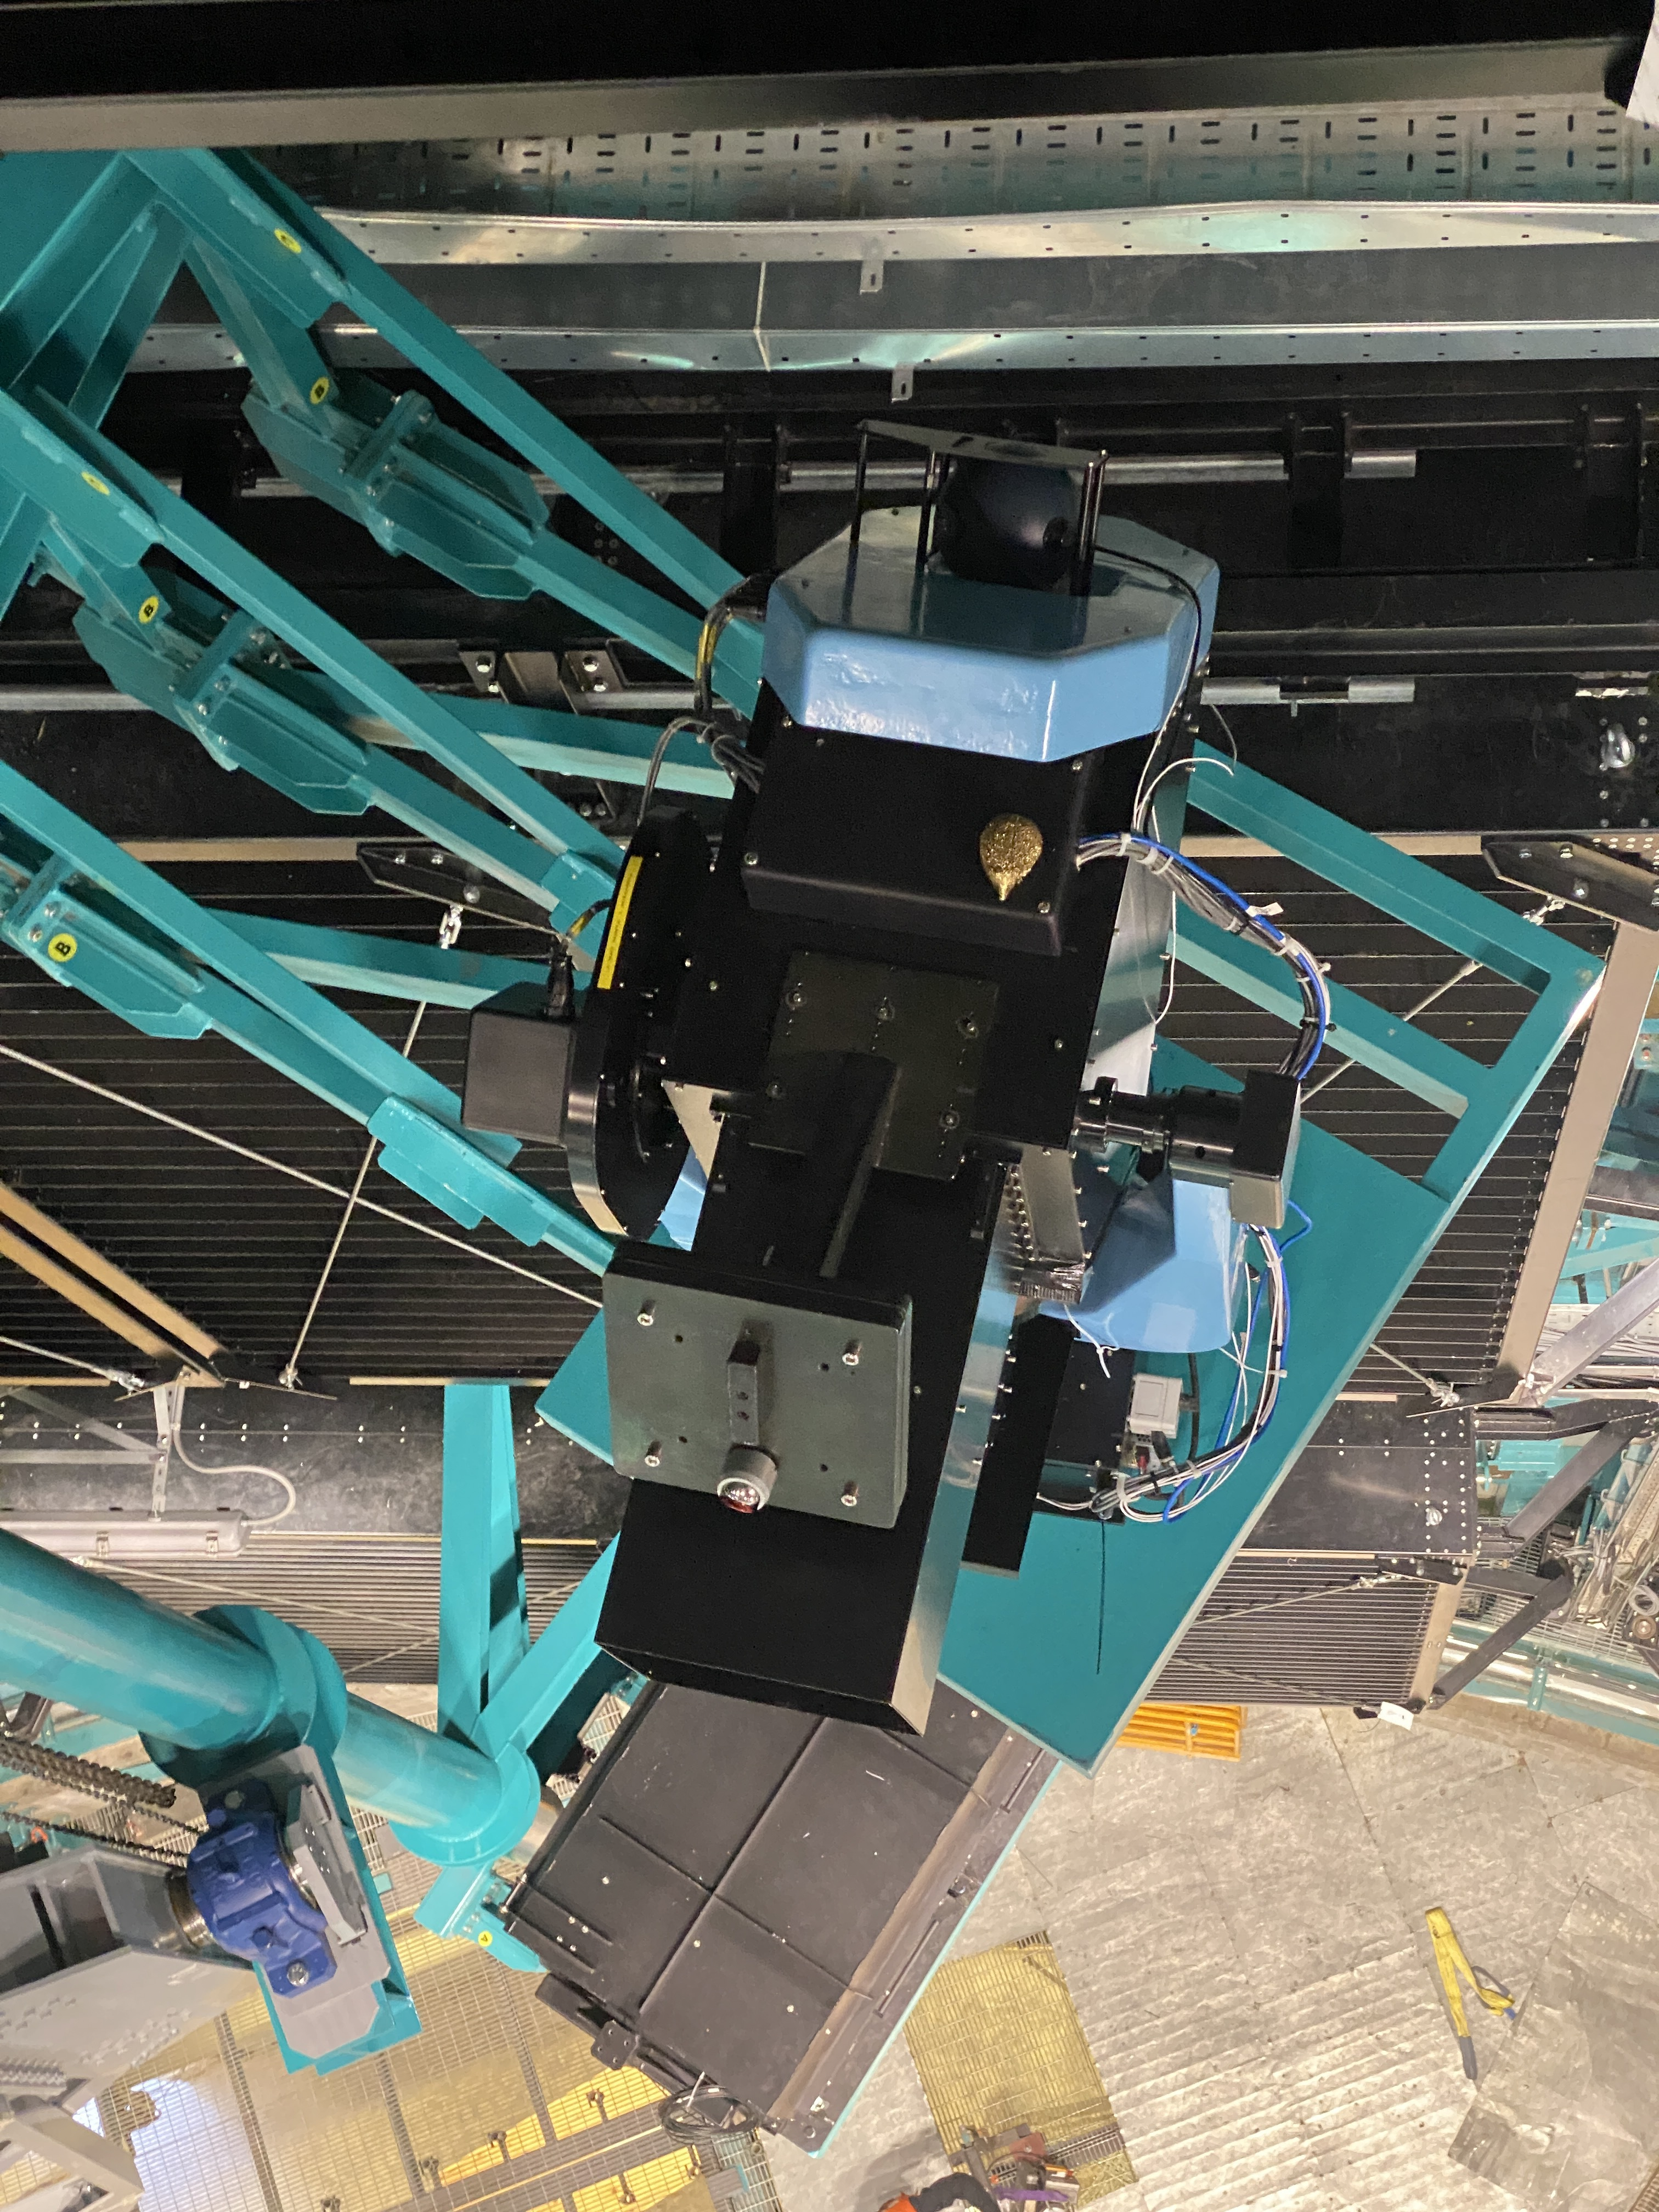
\includegraphics{throughput_for_focused_light_figures/cbp_on_dome_1.png}
  \caption{Image of the CBP, which was installed on the dome on November 22.}
  \label{fig:cbp_1}
\end{figure}
  
\begin{figure}
  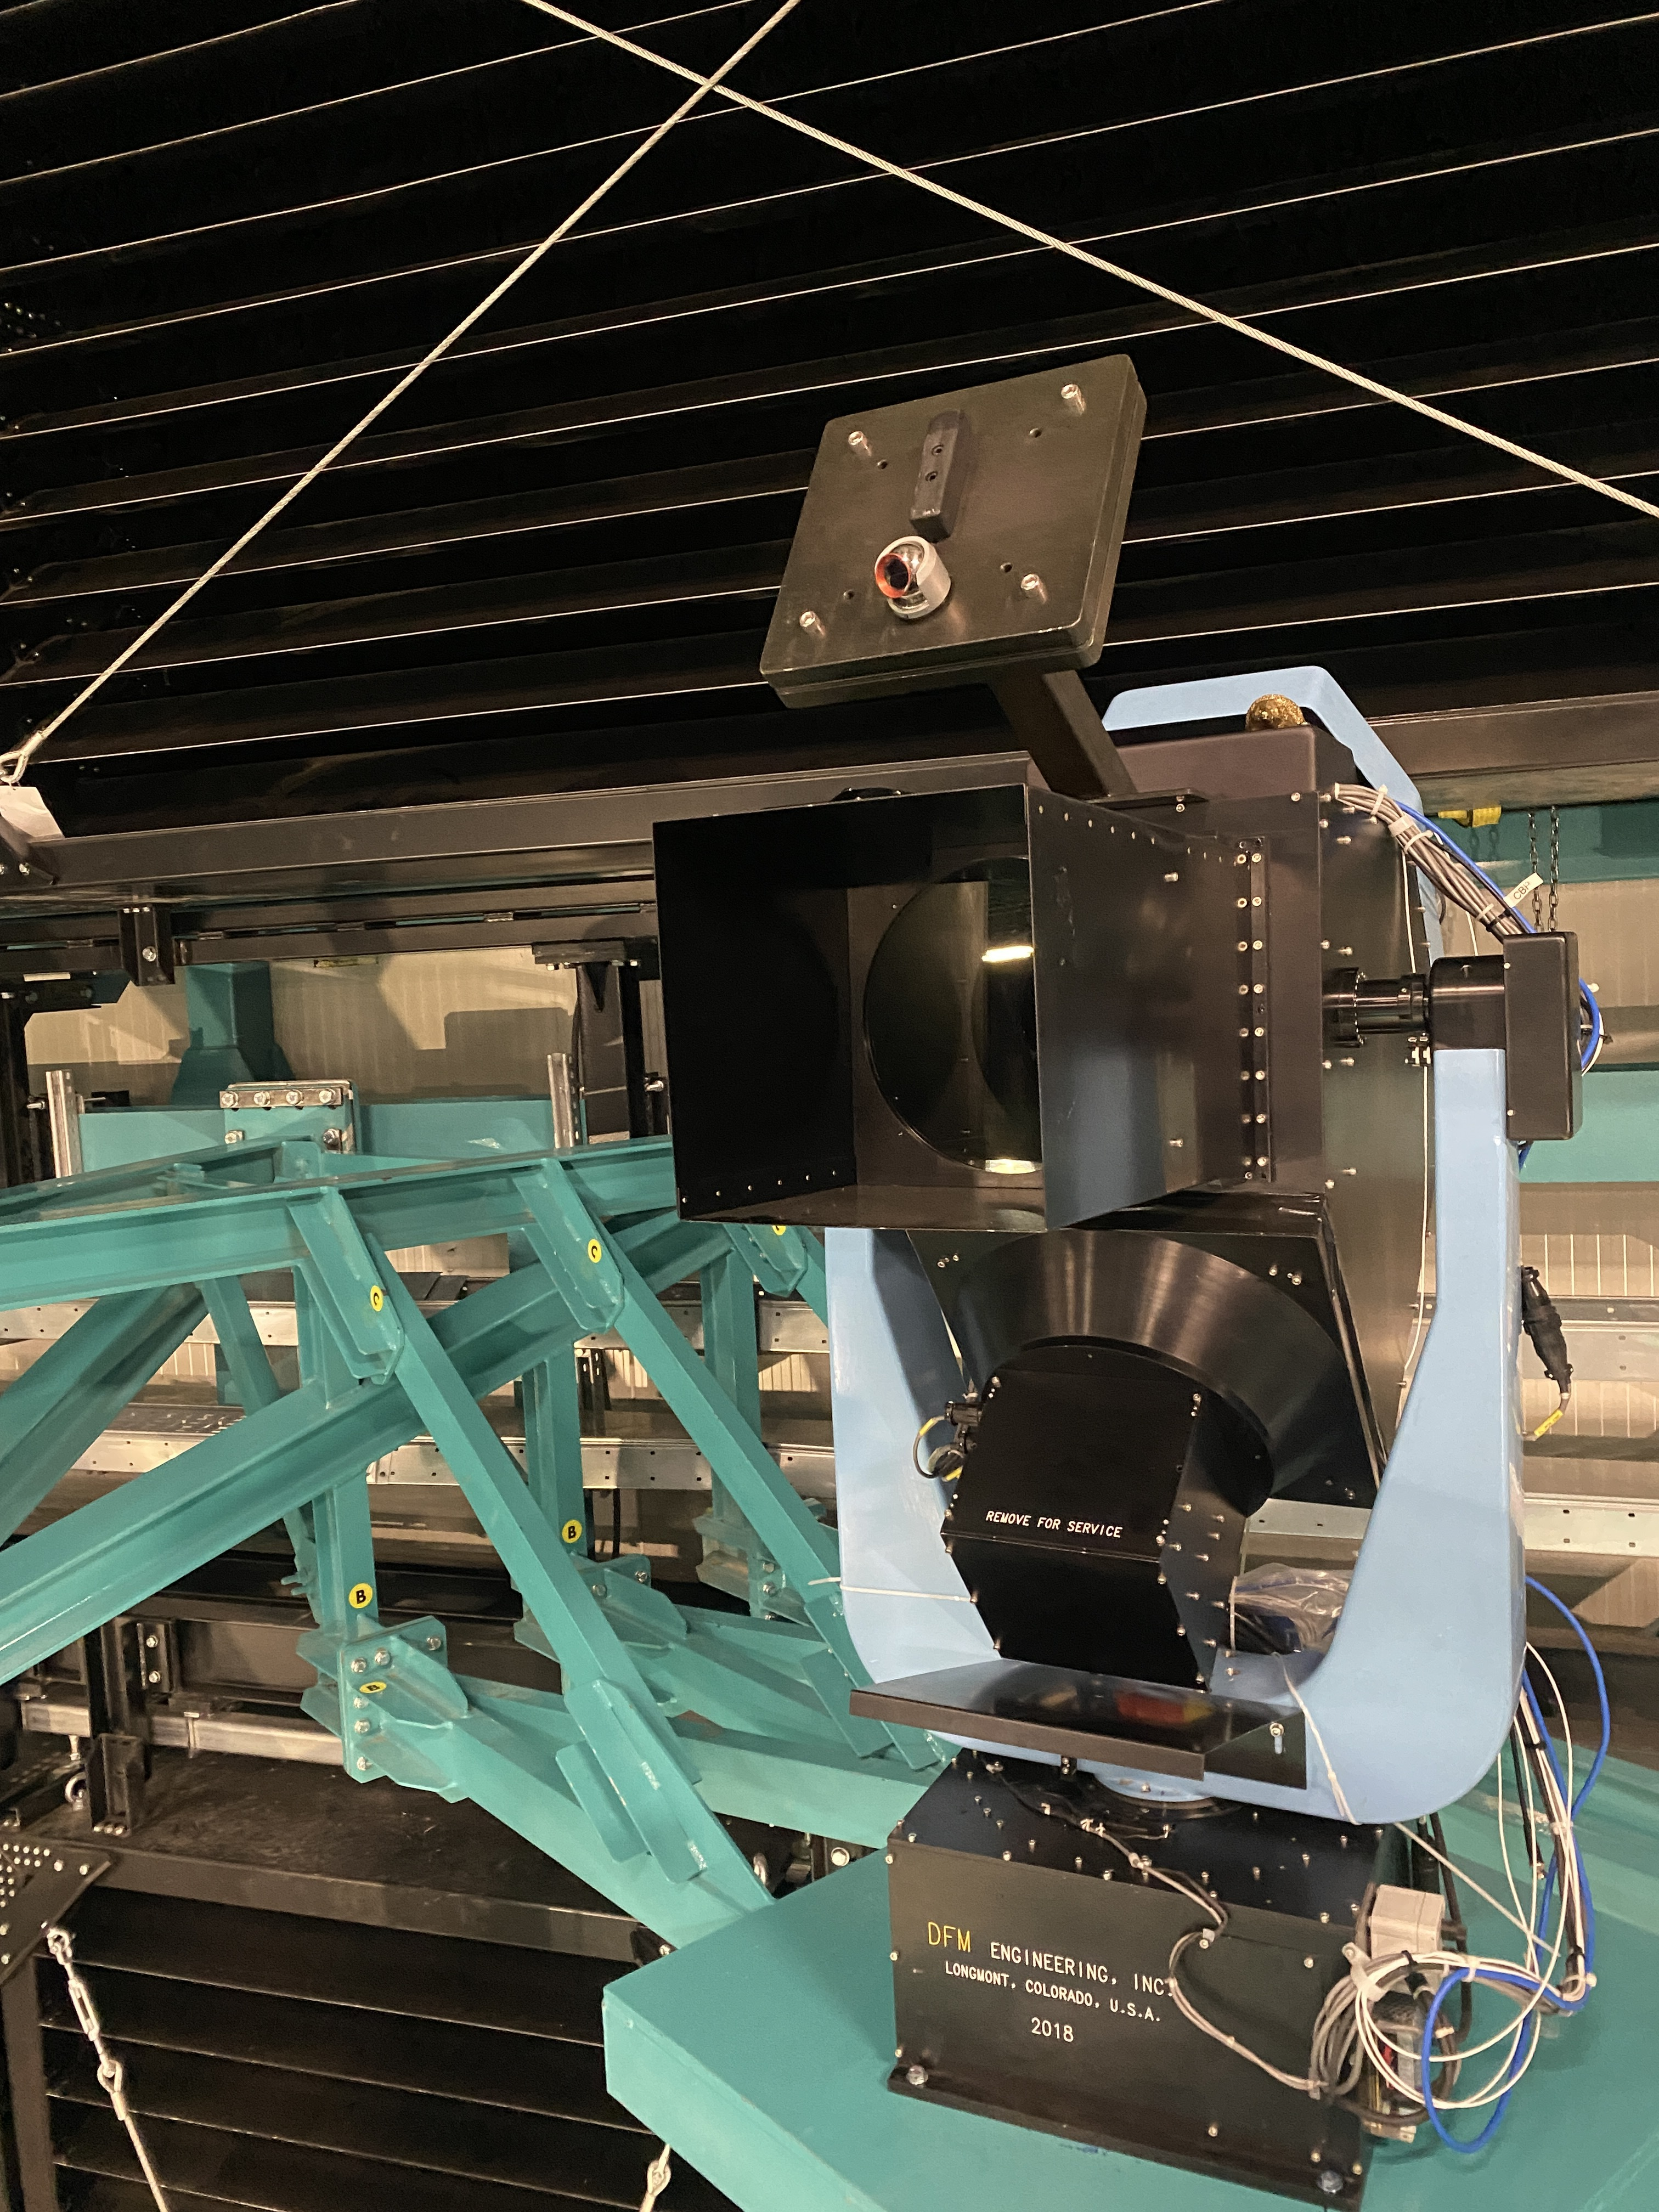
\includegraphics{throughput_for_focused_light_figures/cbp_on_dome_2.png}
  \caption{Image of the CBP, which was installed on the dome on November 22.}
  \label{fig:cbp_2}
\end{figure}
  
\begin{figure}
  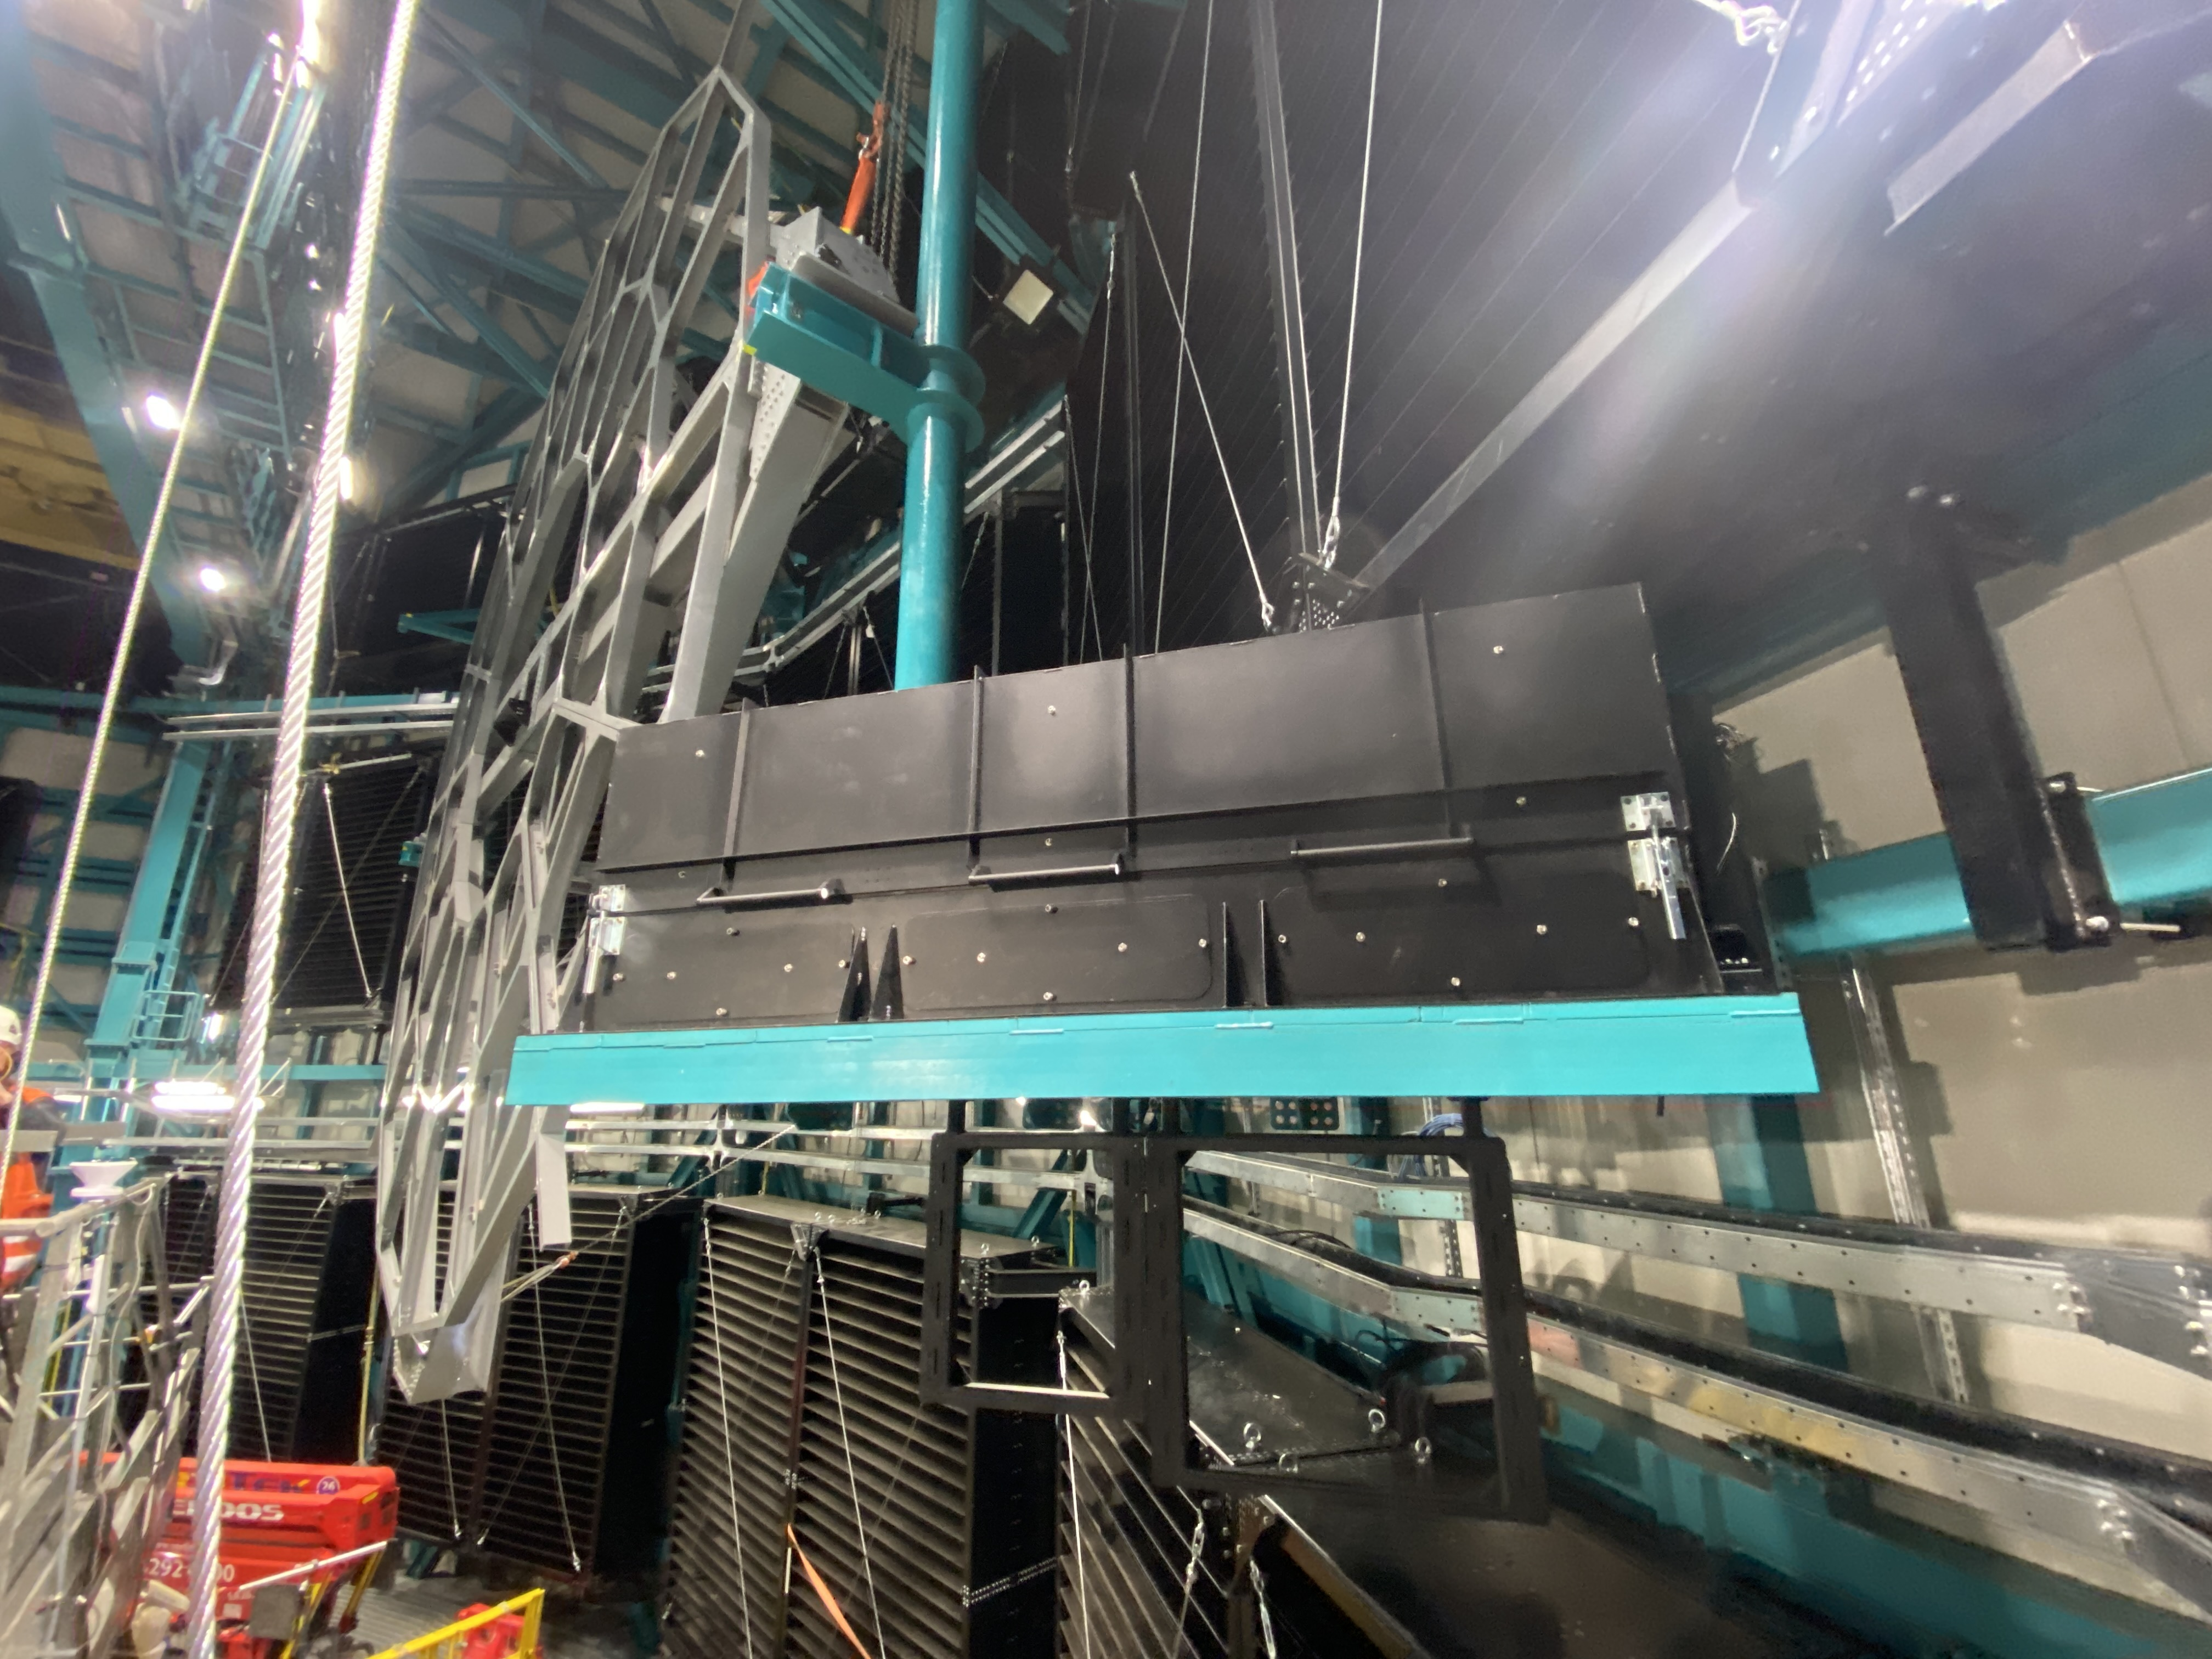
\includegraphics{throughputhroughput_for_focused_light_figures/laser_on_dome.png}
  \caption{Image of the laser box, containing the Ekspla tunable laser, which was installed on the dome on November 21.}
  \label{fig:laser}
\end{figure}

\section{Delivered Image Quality and PSF}
\label{sec:delivered_image_quality_and_psf}


Image quality and PSF modeling are closely tied to the progress of the AOS system, and here is what can be concluded halfway through the data gathering with \ComCam. \\

\textbf{On Image Quality:} \\

The best image quality achieved so far is 0.7 arcsec, with a median of 1.1 arcsec during science visits. As shown in Table \ref{tab:psf_summary} and Figure \ref{seeing_plot}, the PSF FWHM as a function of observation dates highlights the progress. It is important to note that all these data were collected during the AOS testing and validation phase. This makes the achieved image quality even more encouraging, demonstrating significant progress.

\begin{figure*}
        \centering
        \includegraphics[width=\textwidth]{figures/seeing}
        \caption{\small PSF FWHM as a function of the observed date. Data are from DRP from 2024-11-01 to 2024-11-28.}
        \label{seeing_plot}
\end{figure*}


\begin{table*}
\centering
\begin{tabular}{@{}lccc@{}}
\textbf{Filter} & \textbf{Number of Visits} & \textbf{Mean PSF FWHM} & \textbf{STD PSF FWHM} \\ 
All           & 775                      & 1.12                   & 0.23                  \\
u             & 28                       & 1.49                   & 0.08                  \\
g             & 86                       & 1.07                   & 0.14                  \\
r             & 307                      & 1.18                   & 0.22                  \\
i             & 203                      & 1.09                   & 0.24                  \\
z             & 85                       & 1.01                   & 0.21                  \\
y             & 66                       & 1.04                   & 0.18                  \\ 
\end{tabular}
\caption{Summary of PSF FWHM statistics. Data are from DRP from 2024-11-01 to 2024-11-28.}
\label{tab:psf_summary}
\end{table*}


\textbf{On PSF Modeling:}

Two different PSF models are currently used in the DM pipeline: PSFEx, which provides a fast preliminary PSF estimation, and Piff, used later in the pipeline for more accurate PSF modeling. During the initial data collection with \ComCam and AOS testing, most in-focus star shapes exhibited doughnut-like patterns, reflecting residual optical aberrations that had not yet been corrected. This specific form of asymmetry posed challenges for PSF modeling and was not typical. Interestingly, Piff, despite being the more advanced model, struggled to handle the large, non-symmetric PSFs compared to PSFEx. Fig. \ref{growth_plot} shows how we were able early in the observation to constrain the PSF.


\begin{figure*}
        \centering
        \includegraphics[scale=0.2]{figures/curveOfGrowth_pfsex_u_laurenma_DM-30993_LSSTComCam_2024102900140_4}
        \caption{\small Growth curves of the PSF compared to its model (PSFex here)  in the early data taken with \ComCam. }
        \label{growth_plot}
\end{figure*}



However, as the AOS system improved image quality and produced more symmetric PSFs, we observed behavior more consistent with expectations for both PSFEx and Piff. 
Analysis of second-moment reconstructions shows that PSFEx has a systematic offset in size reconstruction compared to Piff, which aligns with observations from DES. Overall, Piff demonstrates better PSF reconstruction, as illustrated in Fig. \ref{DT_plot}. 

\begin{figure*}
        \centering
        \includegraphics[scale=0.47]{figures/0_dT_1d_Piff}
        \includegraphics[scale=0.47]{figures//0_dT_1d_PSFex}
        \includegraphics[scale=0.3]{figures/0_dT_2d_Piff}
	\includegraphics[scale=0.3]{figures/0_dT_2d_PSFex}
        \caption{\small Size residuals for Piff and PSFex (1d distribution and 2d average across visits). Piff has no offset and smaller scatter. Both panels 
        exhibit spatial structure across the focal plane, based on spatial averages across all science visits. The PSF is modeled per CCD in pixel coordinates 
        using a second-order polynomial for interpolation. The observed structure is unlikely to result from atmospheric or dome effects, given that this plot 
        represents an average across visits. Instead, it likely reflects spatial variations not captured by the second-order polynomial interpolation, such as 
        optical aberrations or sensor anomalies.}
        \label{DT_plot}
\end{figure*}


\textbf{On Understanding PSF Physics:}


With LSSTCam, we aim to leverage wavefront sensor data to estimate the optical system's current state and model the optical contribution to the PSF, ultimately building a physical PSF model. During AOS testing with ComCam, the optical state was estimated using out-of-focus images to predict the optical contribution to PSF shape. A ray-tracing analysis showed that the optics fitted from these images could predict the PSF shape, providing strong evidence that a physical PSF model could be developed for LSSTCam (See  Fig. \ref{PSF_plot})


\begin{figure*}
        \centering
        \includegraphics[scale=0.47]{figures/plot_psf_1}
        \includegraphics[scale=0.47]{figures/plot_psf_2}
        \includegraphics[scale=0.47]{figures/plot_psf_3}
        \caption{\small In-focus stars and prediction from the ray tracing on predicting PSF shape (red-dot). Optics parameters on the ray tracing side were derived from out of focus images by measuring optical aberration on "donuts" (out of focus star).}
        \label{PSF_plot}
\end{figure*}

% We’re writing a tech note (SITCOMTN-149) to capture our
% understanding of the state of the system during on-sky commissioning
% campaign with ComCam.  Please use this ticket to capture the work.
%
% From the introduction:
%
% The Vera C. Rubin Observatory on-sky commissioning campaign using
% the Commissioning Camera (ComCam) began on 24 October 2024 and is
% forecasted to continue through mid-December 2024. This interim
% report provides a concise summary of our understanding of the
% integrated system performance based tests and analyses conducted
% during the first weeks of the ComCam on-sky campaign. The emphasis
% is distilling and communicating what we have learned about the
% system. The report is organized into sections to describe major
% activities during the campaign, as well as multiple aspects of the
% demonstrated system and science performance.
%
% Charge:
%
% The groups within the Rubin Observatory project working on each of
% the activities and performance analyses are charged with
% contributing to the relevant sections of the report. The anticipated
% level of detail for the sections ranges from a paragraph up to a
% page or two of text, depending on the current state of
% understanding, with quantitative performance expressed as summary
% statistics, tables, and/or figures.  The objective for this document
% is to summarize the state of knowledge of the system, rather than
% how we got there or “lessons learned”. The sections refer to
% additional supporting documentation, e.g., analysis notebooks, other
% technotes with further detail, as needed. Given the timelines for
% commissioning various aspects of the system, it is natural that some
% sections will have more detail than others.

\section{Instrument Signature Removal}
\label{sec:isr}
\newcommand{\czw}[1]{
  \textbf{CZW: }\textcolor{red}{#1}
}
The quality of the instrument signal removal (ISR) has improved during commissioning, as we create and deploy updated calibration products that better represent the LSSTComCam system.
The following discussion summarizes our current understanding of a variety of features, both expected and newly seen on LSSTComCam, and presents our expected prognosis of the behavior of the full LSSTCam.,

\subsection{Phosphorescence}

There are regions on some of the detectors (most visible in \czw{R22_S01}) which show bright emission, particularly at bluer wavelengths, as shown in Figure \ref{fig:isr_phosphorescence_example}
This is believed to be caused by a thin layer of remnant photo-resist from the manufacturing process that remained on the detector surface, and is now permanent due to the subsequent addition of the anti-reflective coating.
This material is known to be phosphorescent, explaining why these regions show more strongly in the blue.

The initial studies of this (Figure \ref{fig:isr_phosphorescence_decay} show that these features can continue to emit light up to \czw{N seconds} after they've been illuminated.
Due to the long duration of these features, we decided to place manual defect masks over the worst regions, and 

\begin{figure}
  \caption{The phosphorescence seen in \czw{R22_S01}, shown here in a DARK exposure taken after a series of twilight flats (exposure=2024112000065).  This material absorbs light at bluer wavelengths and re-emit that energy over a wide range of wavelengths, and for \czw{add some characterization of the time scales}.}
  \ref{fig:isr_phosphorescence_example}
\end{figure}

\begin{figure}
  \caption{Brightness of a phosphorescent area (defined as \czw{XYZ}) as a function of time since the last illumination, in a series of \czw{bias?} exposures.  Measured by \czw{I remember seeing this, but don't remember who}.}
  \ref{fig:isr_phosphorescence_decay}
\end{figure}

Expected loss ~3.5\%, consistent with estimates of ``less than an amplifier.'' 
The LSSTCam ITL detectors are believed to have been cleaned better, but this may still be an issue.
  
\subsection{Vampire pixels}

Bright pixel with axisymmetric ``depressed'' region.
Appear to conserve charge.
More common than thought.  We're masking with 200\%-of-flat threshold, with X pixel radius circle masks
Two detectors in the full camera may have this at the level of R22_S10.
All ITL have a few.

\begin{figure}
  \caption{A close up of one of the largest vampire pixels.}
\end{figure}

\begin{figure}
  \caption{A view of detector \czw{R22_S10}, which has a large number of less significant vampire pixels.}
\end{figure}


\subsection{Saturated star effects}

Saturated stars end up with dark trails that stretch to the top and bottom of the detector (across channel stops)
Masking will be the solution here as well.  Saturation threshold + width configurations.

\begin{figure}
  \caption{Example of a bright star with full-detector bleed.}
\end{figure}

\subsection{Gain ratios}
We have different observed gain ratios between the lab data and the on-sky data.
Two lab scans come up with different results, and on sky is different still.
Does not seem to correlate with REB temperature, time, VBB etc.
It does appear to be stable, as we've only needed to apply the correction once.

\begin{figure}
  \caption{Example of gain ratio mismatch.}
\end{figure}

\begin{figure}
  \caption{measured ratios}
\end{figure}

\subsection{Crosstalk}

Crosstalk is treated reasonably well by the current set of coefficients: averaged ITL measurements taken on LSSTCam.
Expect those measurements (specifically the filtered version to exclude outliers) will be sufficient at the start of LSSTCam comissioning.
\czw{I want to have numbers and figures here.}

\subsection{Twilight flats}

Twilight flats have worked better than expected.
We now have at least an initial set of flats for ugrizy.
Star print through is one problem we've seen, but this will improve as we take more data + rotations + etc.
Vampire pixels do show up



\section{Low Surface Brightness}
\label{sec:low_surface_brightness}

This update on astrometry quality is based on data collected halfway through the \ComCam observations. It is important to note that so far only single frame astrometric calibration is being done. Doing the additional global astrometric calibration with GBDES will further improve the results presented here.


For now, metrics like AM1 (the RMS of distances between star pairs separated by 5’ across all visits on a tract) appear to be satisfactory. On average, the median value across different filters is around 10 mas, as shown in \figRef{AM1_plot}.

\begin{figure*}
        \centering
        \includegraphics[width=0.7\textwidth]{figures/11d0c9f8-45f6-4bf2-871a-56e00e62060c}
        \caption{\small Stellar Astrometric repeatability in filter I in a given tract. AM1, which is the median of the orange histogram,  is below 10 mas.}
        \label{fig:AM1_plot}
\end{figure*}

When examining the average astrometric residuals projected across the focal plane, some structures appear to be present, as in the example below in \figRef{fov_astrometry_plot}. However, more data is needed to confirm whether these patterns are noise or systematic effects. It is likely that GBDES will help address these structures once it is activated.

\begin{figure*}
        \centering
        \includegraphics[width=0.7\textwidth]{figures/e3aea76f-3ed1-4686-9a24-00abf0ff9515}
        \caption{Declination residuals projected in Focal plane coordinate for a given tract. Some structure looks to be present in focal plane coordinates, which will be taken into account with GBDES. }
        \label{fig:fov_astrometry_plot}
\end{figure*}


\section{Photometric Calibration}
\label{sec:photometric_calibration}

We have started commissioning the full photometric calibration pipeline for
Rubin Observatory, with great success so far. For testing photometric
calibration we have obtained over 150 dithered science observations in ugriz
over the Extended Chandra Deep Field-South (ECDFS) (one of the planned LSST
deep fields), and tens more in rizy over the Euclid Deep Field South
(EDFS). All of the science data has delivered seeing of $\sim0.8$ to $\sim1.5$
arcsecond seeing, which is due to the excellent work of the AOS team.  The
validation work in this document covers the ECDFS field with more complete
filter coverage.

The precision photometric calibration software used for Rubin is the Forward
Global Calibration Method (Burke, Rykoff, et al. 2018) which was used
successfully to achieve better than 2 mmag uniformity for the Dark Energy
Survey. This software has been adapted for the LSST Science Pipelines and has
been used on Hyper Suprime Cam Special Survey Program (HSC SSP) for data
releases since DR2.

The performance on HSC data has not been as good as that on DES data due to a
number of reasons, yielding repeatability and uniformity closer to the 5 mmag
level for grizy data.  First, we have had a lot of problems with HSC
backgrounds and amp-to-amp non-linearities.  Second, the HSC survey strategy
was not well suited to self calibration due to the slow slewing of the
telescope and the long time required to change a filter, leading to lots of
isolated single-band single-night surveys.  Third, we do not have detailed
throughput scans including detector-to-detector QE variations and in-situ scans
of the significant filter variations that are required for the full forward
modeling in FGCM.

Early calibration of the ComCam data is in many ways easier than that of HSC.
First of all, we have a smaller camera (9 detectors) and thus fewer variations
to have to cross-calibrate.  Second, the camera is situated in the center and
easiest to calibrate part of the focal plane.  Third, we only have one field to
calibrate across a few nights of data so far over a limited range of airmass.
Fourth, the survey strategy (multiple bands per night dithered and repeated
with overlapping filters from night to night) is well suited to
self-calibration.  On the other hand, we do not have the CBP set up yet, so we
do not have detailed filter or detector scans available for ComCam, and are
just using the LSSTCam reference filter throughputs and average detector
throughput for the LSSTCam ITL detectors.  In addition, we do not have a flat
field screen so we have had to rely on twilight flat observations for flat fielding.

\subsection{Processing Overview}

We start with the standard ISR as documented in Section~\ref{sec:isr}. While
there are a number of challenges that we have discovered with the ITL
detectors, these are mostly near the sky level, while the testing of
photometric calibration is focused on brighter stars that are less affected by
these issues. We then apply twilight flats, which we are investigating how to
make better. At the same time, we are going to have the flat field screen and
laser and projector installed prior to the commissioning of LSSTCam, so we do
not want to spend too much time worrying about specific challenges of twilight
flats which are only necessary for ComCam.

After flat fielding we find an initial point-spread function (PSF), do a star
selection based on source and psf moments that was developed for HSC
single-frame processing, and perform an initial astrometric solution and
photometric solution (with a single zero-point per detector).  The initial
astrometric solution is used to associate star observations together prior to
global photometric calibration with FGCM.  The initial photometric solution is
used for rapid analysis and prompt processing, but is not used at all for FGCM
which relies entirely on instrumental fluxes (in units of electrons) with a
minor constraint from the reference catalog.

\subsection{Global Photometric Calibration with FGCM}

All associated stars with observations with signal-to-noise greater than 10 are
input into the FGCM solution.  In addition, reference stars from The Monster
reference catalog are associated with the stars .  Only a small fraction of the
reference stars are used in the FGCM solution, sufficient to estimate an
``absolute'' calibration (trusting that The Monster is a good absolute
reference catalog).  There is additional ongoing work with absolute calibration
with respect to the CalSpec star C26202 which is not saturated in LSST images
and is fortunately contained in ECDFS that is described below.

The FGCM model constrains the atmospheric parameters per night, as well as the
absolute throughput relative to the input scans.  The standard atmosphere is
given by MODTRAN, run at the elevation of Cerro Pachon at airmass 1.2 with an
Angstrom aerosol model.  The optics and filters are all taken from
$lsst/throughputs$ version 1.9, and the detector throughput is taken from the
ITL average of the lab scans ingested into $obs\_lsst\_data$.  Note that the
detector QEs are normalized to 1.0 at 800 nm, which is certainly
greater than the true QE at this wavelength.



\section{Survey Performance}
\label{sec:survey_performance}

Understanding and predicting survey performance includes modeling the likely input telemetry, the expected performance of the telescope and observatory, as well as understanding the survey strategy and its interaction with science outcomes. 

At this point in commissioning, the operations of the observatory are focused on obtaining specific observations, with very different strategies than will be employed during operations. This includes very different configurations of the Feature Based Scheduler. Thus, we are not testing the Feature Based Scheduler as it would be used in operations yet, and have no comment about issues that may be related specifically to survey strategy implementation. 

We can however begin to evaluate how our models may be validated or not by the currently acquired observations. We focus on the observations acquired for the science program, BLOCK-320.

First, clearly bad visits (where stars were clearly trailed in the images, as visible in rubintv) were removed from the set of science visits. 

The throughput curves available in `syseng_throughputs`, the repository that tracks current system engineering summaries of full-focal-plane throughputs, can be used to predict zeropoints for average ITL CCDs. See \url{https://github.com/lsst-pst/syseng_throughputs/blob/main/notebooks/InterpolateZeropoint.ipynb}, where a simple interpolation function for filter and airmass is defined for the current throughputs (v1.9). The returned zeropoint includes the exposure time, as zeropoints in DM pipelines outputs are for a given exposure with the given exposure time (they are not 1-second zeropoints). A comparison of these predicted zeropoints to the reported median visit zeropoints in the ConsDB (the column `cdb_lsstcomcam.visit1_quicklook.zero_point_median`) is shown in Figure~\ref{fig:zeropoints). The mean of these zeropoint variations averages 0.13 magnitudes across all bands, being slightly smaller in r (0.09 mag) and slightly larger in y band (0.18); the RMS scatter in these measurements is < 0.02 magnitudes. 

\begin{figure}
    \centering
    \includegraphics[width=0.8\textwidth]{sp/zeropoints.png}
    \caption{Predicted zeropoints from syseng_throughputs (accounting for airmass) compared to measured zeropoints from `cdb_lsst.comcam.visits1_quicklook`.}
    \label{fig:zeropoints}
    \end{figure}

\section{Sample Production}
\label{sec:sample_production}

\section{Difference Image Analysis: Transience and Variable Objects}
\label{sec:dia_transient_variable}

\section{Difference Image Analysis: Solar System Objects}
\label{sec:dia_solar_system}

\subsection{Galaxy Photometry}
\label{sec:galaxy_photometry}

Galaxy photometry investigations so far have used the Extended Chandra Deep Field-South (ECDFS) due to the availability of public external reference data, including space-based imaging from the Hubble Space Telescope (HST).
Broadly, we have done (or soon will be doing) comparisons to matches against external catalogs and from synthetic source injection (SSI) in coadds.
Some preliminary investigations were done with visual inspection of external images.

\iffalse                                % doesn't appear to have added much to ComCam analysis
\subsubsection{Comparison to External Imaging}
\label{subsec:galaxy_photometry_external_imaging}

We downloaded a subset of the Hubble Legacy Fields (HLF, \url{https://archive.stsci.edu/prepds/hlf/}) imaging for the GOODS-South field, which included programs covering the original Chandra Deep Field-South and parallel fields now part of ECDFS.
Significantly overlapping coverage is available in F435W, F606W, F775W and F814W, as well as four redder bands.
F775W is of particular interest for galaxy photometry since it was designed to match the SDSS i-band filter.

Visual inspection of a particular group of photogenic galaxies in the HST imaging revealed an excess point source in the ComCam imaging from Nov. 8, which was subsequently found to match the position of an alert issued by several ZTF brokers in early September.
We experimented with using the HST image as a template for difference imaging by PSF matching and resampling to ComCam resolution.
This can be done relatively successfully on a per-object basis, but unfortunately, the image registration/warping for the HST images is too inconsistent to make it worthwhile on patch scales without re-warping one image or the other.

Besides visual inspection, no other uses of or comparisons to external imaging have yet been demonstrated.
DM-47576 (\url{https://rubinobs.atlassian.net/browse/DM-47576}) has been informally assigned to an in-kind contributor to make loading and displaying HST images more convenient should a need arise.

Joint modelling of space and ground imaging has been demonstrated with MultiProFit in COSMOS with the Subaru Hyper Suprime-Cam (HSC) and HST data on DM-46497 (\url{https://rubinobs.atlassian.net/browse/DM-46497}) but has not been attempted with ComCam data and is not considered a high priority, in part due to the aforementioned astrometry/warping issues.
\fi

\subsubsection{Comparison to External Catalogs}
\label{subsec:galaxy_photometry_external_catalogs}

DM-47234 (\url{https://rubinobs.atlassian.net/browse/DM-47234}) compared the tract 5063 20241120 DRP object table galaxy photometry with the latest HLF and Dark Energy Camera Legacy Survey DECaLS (DECaLS, \url{https://www.legacysurvey.org/decamls/}) catalogs.

\begin{figure}
  \includegraphics{galaxy_photometry/cdfs_i_vs_HST_F775W.png}
  \caption{Difference between i-band CModel magnitudes and HST F775W magnitudes in ECDFS.}
  \label{fig:cdfs_i_vs_HST_F775W}
\end{figure}

\figRef{cdfs_i_vs_HST_F775W} shows difference between i-band CModel magnitudes and the HLF HST F775W SourceExtractor magnitudes for both stars and galaxies, using the HST star-galaxy classification.
The median difference in both stellar and galaxy photometry is fairly flat across 19<i<25, but also quite large at about 175 mmag for galaxies and 75 mmag for stars.
Presuming that the difference in stellar photometry is mainly a calibration issue, the differential between galaxies and stars is still more than a factor of 2 (and still more in quadrature).
This could be due to differences in methodology; the HST SourceExtractor-derived magnitudes are more like aperture photometry than a model fit.

\begin{figure}
  \includegraphics[width=0.5\textwidth]{galaxy_photometry/cdfs_g_vs_DECaLS.png}
  \includegraphics[width=0.5\textwidth]{galaxy_photometry/cdfs_g_vs_desy3g.png}
  \caption{Difference between g-band CModel magnitudes and DECaLS/DES-Y3G catalog values in ECDFS.}
  \label{fig:cdfs_g_vs_des}
\end{figure}

\figRef{cdfs_g_vs_des} shows the difference between g-band CModel magnitudes and measurements from two Dark Energy Survey (DES) DECam (Dark Energy Camera)-based catalogs.
The DECaLS (Dark Energy Camera Legacy Survey) DR10 processing is more recent and includes model photometry, selecting the least complicated model required to provide a good fit from a PSF to a single free Sersic fit.
The Dark Energy Survey Year 3 Gold (DES-Y3G) sample is an older, shallower dataset, albeit using pipelines more similar to the ComCam/DRP pipelines.
The median difference between stellar magnitudes is relatively small but varies with magnitude and between the two catalogs.
However, given the difference between filters and that no color term corrections have been applied, both the medians offset and scatter of 10 to 30 mmag are acceptable.
Bright ($g < 20.3$) galaxies have median offsets smaller than 10 mmag and scatter of 82 and 64 mmag in DECaLS and DES-Y3G, respectively.

\begin{figure}
  \includegraphics[width=0.5\textwidth]{galaxy_photometry/cdfs_r_vs_DECaLS.png}
  \includegraphics[width=0.5\textwidth]{galaxy_photometry/cdfs_r_vs_desy3g.png}
\caption{Difference between r-band CModel magnitudes and DECaLS/DES-Y3G catalog values in ECDFS.}
  \label{fig:cdfs_r_vs_des}
\end{figure}

\figRef{cdfs_r_vs_des} shows r-band magnitude difference plots.
Here, the median difference for stars are magnitude-dependent in both catalogs, suggesting that color terms are more important.
Similarly, the scatter is much larger, at about 80mmag for $r < 20$.
However, the magnitude dependence in the median difference is stronger in DECaLS, both for stars and galaxies.
Inspection of the $g-r$ versus $r-i$ stellar locus plot (not shown) reveals that DECaLS photometry has a substantial fraction (about 10\%) of outliers, some even a full magnitude off the stellar locus.
At any rate, the scatter in galaxy magnitudes is not much larger than that for stars (in fact, it is noticeably smaller in DES-Y3G).
Additionally, in DES-Y3G, the median magnitude difference is fairly flat for $19<r<23$, so despite the numerous differences in hardware and software, the two catalogs are not inconsistent.
The i-band photometry in DECaLS shows qualitatively similar but quantitatively worse pathologies and is omitted for brevity.

\begin{figure}
  \includegraphics[width=0.5\textwidth]{galaxy_photometry/cdfs_g_vs_rmi_DECaLS.png}
  \includegraphics[width=0.5\textwidth]{galaxy_photometry/cdfs_g_vs_rmi_desy3g.png}
\caption{Difference between $r-i$ CModel colors and DECaLS/DES-Y3G catalog values in ECDFS.}
  \label{fig:cdfs_rmi_vs_des}
\end{figure}

The $r-i$ color differences shown in \figRef{cdfs_rmi_vs_des} are similar between all three catalogs.
The median differences are very small, albeit different in sign between the two pairs of catalogs.
The scatter in star color differences is nearly constant to about 22nd magnitude, whereas for galaxies it scales with signal-to-noise to a minimum of about 25mmag at 20th mag (photometry for brighter galaxies is limited by model inadequacy and irregular structure).
In short, galaxy colors appear quite consistent between all three catalogs, although how the small differences impact derived quantities like photometric redshifts remains to be seen.

\subsubsection{Additional Investigations}
\label{subsec:galaxy_photometry_additional}

Analysis of the accuracy of magnitude and color errors await the implementation of synthetic galaxy injection in DM-47185 (\url{https://rubinobs.atlassian.net/browse/DM-47185}).
Some analysis is possible with matching to reference catalogs; however, besides the problems with the DECaLS photometry, we are not yet taking into account reported errors on reference fluxes (which may themselves be underestimated).

Besides single-band/forced CModel photometry, MultiProFit multi-band (gri) single Sersic fits have been run on a single patch in tract 5063 on DM-47526 (\url{https://rubinobs.atlassian.net/browse/DM-47526}) but have yet to be analyzed.
Other algorithms like aperture, GaAP and Kron magnitudes/colors have yet to be compared.

\subsubsection{Conclusions}
\label{subsec:galaxy_photometry_conclusions}

Galaxy photometry in ECDFS appears consistent with at least two different catalogs covering the same field (one space based) and the differences identified in a third (DECaLS) appear to be peculiar to that catalog, not our own processing.
This is not to say that the galaxy photometry is optimal, as hardware and software differences make it difficult to quantify expected differences.
Comparisons to external data should be more illuminating once we have coadds in the COSMOS field and can compare to HSC imaging with the same pipeline versions.


\section{Weak Lensing Shear}
\label{sec:weak_lensing_shear}

\section{Crowded Stellar Fields}
\label{sec:crowded_stellar_fields}

The prospects for human-based inspection of the vast number of images to be
produced by the Rubin/LSST are unavoidably going to be limited to a 
fraction of the dataset produced (even nightly, let alone for the full 10-year
survey).  Yet, the potential value of getting human eyes on the images (including
the raw, minimally processed, and final processed and calibrated stages), is
immense, in particular for identifying patterns that are easily spotted by eye,
yet tend to evade most modern automated image quality assessment protocols.

Every dataset from any given observation program comes with its own unique set
of ``features'' stemming from the observatory structures, optics, camera,
detectors, electronics, observation strategy, the night sky, calibration products, 
etc.  This makes eyeball inspection particularly valuable in the early days of 
commissioning.  Fortuitously, the energy and enthusiasm of internal project members
are at extrememly high levels at this stage, so there is no shortage of voluntary
effort for human visial inpsection for the commissioning phase of the \ComCam.
This effort to date has largely proceded via an informal
see-something-say-something scheme, with many users posting their latest findings
on the internal staff Slack channels (namely the \#sciunit-image-inspection channel,
but also prominently in other channels, \#sciunit-lsb, \#validation-team,
\#embargo-beautiful-images, \#ops-satellites, \#dm-calibraion-products to name a few).

Anomolies and peculiarities reported to date along with details of and/or pointers
to further study and explanation (where applicable) include:
\begin{itemize}

\item \textbf{ghosts}: most prominent around bright stars (including those falling
  outside of the FOV) and attributed to multi-bounce reflections off of the focal
  plane and the \ComCam optics.  Qualitatively, the presence and appearance of 
  the ghosts are well predicted by Josh Meyers' ``batoid ray tracer'', even in its
  current unoptimized state.  It is noted that the nature of the ghosts will be
  quite different for the full LSSTCam, but this initial level of understanding
  of this feature is promissing and useful for honing characterization and
  mitigation strategies.

\item \textbf{stray/scattered light}: prominent ring-shaped waffle/corduroy-like
  features seen early on were identified as originating from a blinking light on a
  crane that was left on. Large irregular ring-shaped ``spots'' were attributed to
  the laser tracker (an issue in access to turn it off was noted). \ComCam is 
  known to be less well baffled than LSSTCam, so scattered light from off-axis light 
  sources is expected to be worse.

\item \textbf{satellite streaks}: see Section~\ref{sec:dia_transient_variable}

\item \textbf{kettlebell \& trefoil-shaped PSFs}: see Section~\ref{sec:aos_commissioning}.
  This issue was further investigated in the context of the PSF modelling itself on such
  irregularly shaped PSFs.  It was noted that the preferred ``piff'' algorigthm (which
  is used for the final characterization model) was performing worse that the ``psfex''
  algorithm (which, due to its relative speed, is used in the initial characterization).
  As such, we temporarily switched to using only ``psfex'' until the image quality was
  improved.  Given the incredible and expeditious work of the AOS team, we are already
  confident that we can switch back to our preferred configurartion.  (This has also
  spurred a study into the reason why ``piff'' seems to struggle with these shapes and
  will hopefully lead to improvements there, see
  Section~\ref{sec:delivered_image_quality_and_psf}).

\item \textbf{background subtraction issues}: see Section~\ref{sec:low_surface_brightness}

\item \textbf{repeated patchwork gradients}: a small number of images appear to have a 
  bias gradient that appears in several amplifiers of detector 1 (R00\_S01). This feature 
  is currently under investigation, but it appears to be most prominent when a bright star 
  resides close to the amplifier (right) edge of this detector. The bias shift appears in 
  the prescan, active area, and overscan regions of the affected amplifiers. It seems 
  likely that this is some type of crosstalk, but the origin and manifestation is unclear. 
  It remains to be seen whether similar features are seen in any other detectors. It is 
  likely that this feature will be further studied in the context of Section~\ref{sec:isr}.

\item \textbf{trailed sources}: due to tracking errors.  These are particularly
  difficult to identify with automated image quality metrics (there are some ideas
  about using AI to identify tracking error-based image degradation floating around,
  but we also hope to be able to confidently rely on data from the EDF to indicate
  tracking issues).

\end{itemize}

\noindent \textbf{Future Endeavors}

A major goal for future image inspction efforts is to develop a more systematic
way to identify and report issues and, where possible, alert the
relevant stakeholders for further investigations into mitigating problems.

There has been some effort to deploy the ``Exposure Checker'' that was developed for the Dark Energy Survey \citep{2016A&C....16...99M}\footnote{See demo \url{https://des-exp-checker.pmelchior.net/}} and has been previously deployed by LSST DESC for the visual inspection of simulated DC2 data \citep{2021ApJS..253...31L}.

Also recently implemented for visual inspection is a rendering of the 3-color coadd
HIPS maps produced regularly during the nightly validation and DRP processing runs.
Such images are invaluable for highlighting myriad issues at the coadd level (often
indicating a need to drill-down to the visit-level for a full diagnosis, while
providing significant clues on where to look first).


\appendix
% Include all the relevant bib files.
% https://lsst-texmf.lsst.io/lsstdoc.html#bibliographies
\section{References} \label{sec:bib}
\renewcommand{\refname}{} % Suppress default Bibliography section
\bibliography{local,lsst,lsst-dm,refs_ads,refs,books}

% Make sure lsst-texmf/bin/generateAcronyms.py is in your path
\section{Acronyms} \label{sec:acronyms}
\addtocounter{table}{-1}
\begin{longtable}{p{0.145\textwidth}p{0.8\textwidth}}\hline
\textbf{Acronym} & \textbf{Description}  \\\hline

ComCam & The commissioning camera is a single-raft, 9-CCD camera that will be installed in LSST during commissioning, before the final camera is ready. \\\hline
PSF & Point Spread Function \\\hline
SE & System Engineering \\\hline
\end{longtable}

% If you want glossary uncomment below -- comment out the two lines above
%\printglossaries





\end{document}
